% Compile with xelatex
% Install the Hack font from http://sourcefoundry.org/hack/

\documentclass[10pt,DIV=9]{scrartcl}

\usepackage[english]{babel}
\usepackage[english]{isodate}
\cleanlookdateon

\usepackage{float}
\usepackage{graphicx}
\usepackage{dcolumn}
\newcolumntype{d}[1]{D{.}{.}{#1}}
\usepackage{multirow}
\usepackage{calc}

\usepackage{listings}
\usepackage{fontspec}
\lstset{
  basicstyle=\scriptsize\fontspec{Hack},
  breakatwhitespace=true,
  breaklines=true,
  caption=\texttt{\lstname},
  frame=single,
  showspaces=false,
  showstringspaces=false,
  showtabs=false,
}

\begin{document}

\title{Mesh Network Performance}
\subtitle{Net4D Assignment 2}
\author{Kieren Davies \and Saleem Manjoo \and Jono Schoeman}
\date{\printdate{2016-05-29}}
\maketitle

\section{Task 1: Visualization}

\begin{figure}[H]
  \caption{OLSR with all antennae connected}
  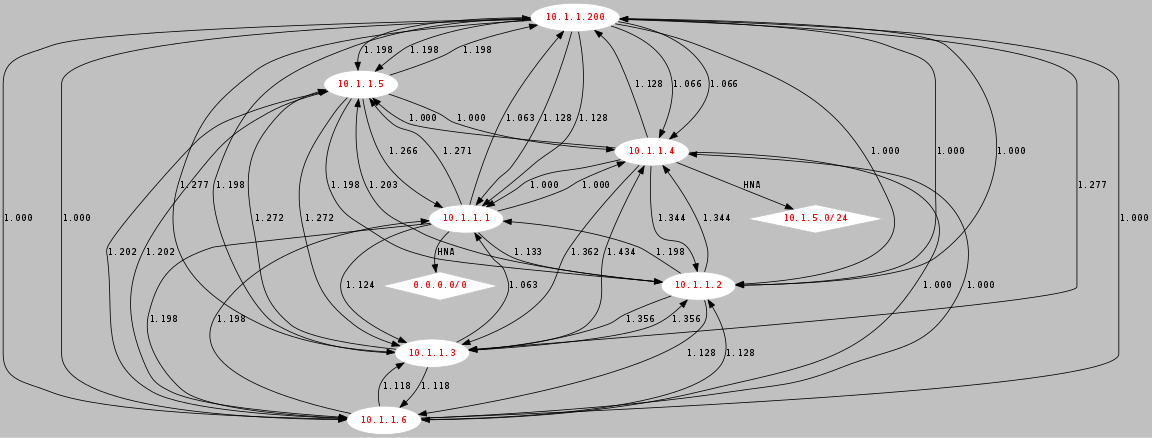
\includegraphics[width=\textwidth]{dot-olsr-full}
\end{figure}

\begin{figure}[H]
  \caption{OLSR with some antennae removed}
  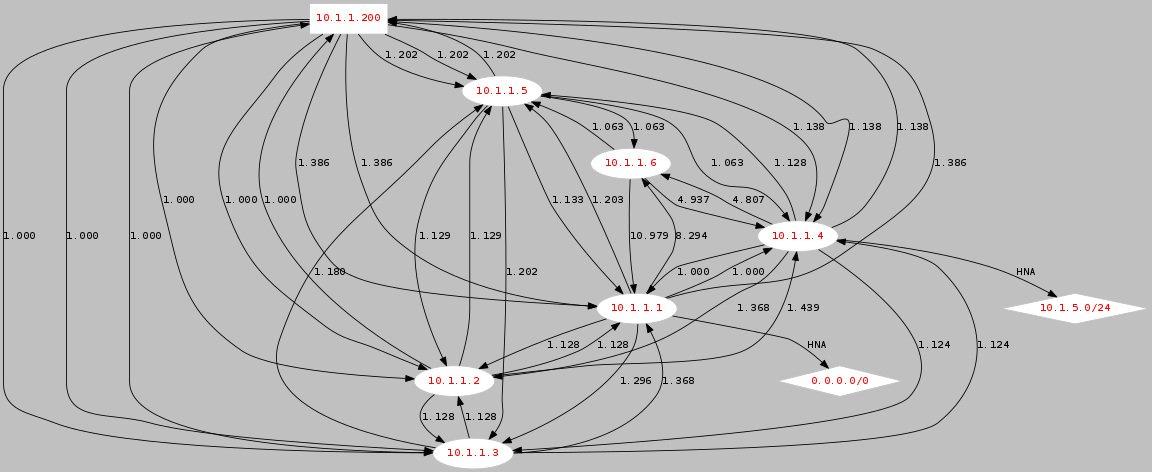
\includegraphics[width=\textwidth]{dot-olsr-partial}
\end{figure}

\section{Task 2: TCP throughput}

Measurements were taken by running \texttt{iperf} in server mode on the gateway node and in client mode on other nodes for 60 seconds each.

\begin{table}[H]
  \caption{TCP throughput}
  \centering
  \begin{tabular}{|r|*{2}{d{2}|}} \hline
    \multirow{2}{*}{Node} & \multicolumn{2}{c|}{Throughput (Mbps)} \\
    & \multicolumn{1}{c|}{\makebox[\widthof{BATMAN}][c]{OLSR}} & \multicolumn{1}{c|}{BATMAN} \\ \hline \hline
    1 & 4.67 & 4.81 \\ \hline
    2 & 4.92 & 5.01 \\ \hline
    3 & 4.94 & 5.03 \\ \hline
    4 & 4.99 & 4.94 \\ \hline
    5 & 5.02 & 4.94 \\ \hline
    6 & 5.04 & 5.11 \\ \hline
    7 & 5.05 & 5.09 \\ \hline
    \hline
    avg & 4.95 & 4.99 \\ \hline
  \end{tabular}
\end{table}

\section{Task 3: Round-trip time}

Measurements were taken by running \texttt{ping} on the gateway node against other nodes for 60 seconds each.

\begin{table}[H]
  \caption{Round-trip time}
  \centering
  \begin{tabular}{|r|*{4}{d{2}|}} \hline
    \multirow{3}{*}{Node} & \multicolumn{4}{c|}{Time (ms)} \\
    & \multicolumn{2}{c|}{\makebox[\widthof{BATMAN}][c]{OLSR}} & \multicolumn{2}{c|}{BATMAN} \\
    & \multicolumn{1}{c|}{avg} & \multicolumn{1}{c|}{max} & \multicolumn{1}{c|}{avg} & \multicolumn{1}{c|}{max} \\ \hline \hline
    1 & 2.62 &  6.60 & 3.07 & 18.89 \\ \hline
    2 & 2.52 &  7.33 & 2.47 &  5.66 \\ \hline
    3 & 3.09 & 22.05 & 2.61 & 15.94 \\ \hline
    4 & 2.53 &  6.56 & 2.75 & 18.46 \\ \hline
    5 & 2.77 & 14.81 & 3.27 & 29.56 \\ \hline
    6 & 2.60 & 25.54 & 2.67 & 11.40 \\ \hline
    7 & 2.35 &  6.52 & 3.01 & 24.57 \\ \hline
    \hline
    avg & 2.64 & 12.77 & 2.84 & 17.78 \\ \hline
  \end{tabular}
\end{table}

\section{Task 4: Route flapping}

The following shell script was used to detect route flapping.  It repeatedly calls \texttt{traceroute} and compares the most recent route to the previous.  A flap is reported if the routes differ.  An asterisk in the output, which indicates a timeout, is not considered a difference.

\noindent
\begin{minipage}{\linewidth}
  \lstinputlisting[language=bash]{flapping.sh}
\end{minipage}

In the first attempt with OLSR, no flaps were detected, since every node had a direct connection to every other node.  We therefore removed the antennae from node 6 in the honours lab, so that only nodes 5 and 7 were within range of it.  We then attempted to detect flapping between the gateway node and node 6.  In one hour, 61 flaps were detected, with one intermediary hop alternating between nodes 5 and 7.

Similarly, in the first attempt with BATMAN, no flaps were detected.  When we removed the antennae of node 6, no route was found to it from the gateway.  We waited half an hour but the route did not repair in this time.

\section{Task 5: Repair time}

We removed antennae from one node at a time in the honours lab, and timed the interval from antenna removal to first successful ping from the gateway to the node.

OLSR repaired in an average of 10.7 seconds.  BATMAN did not repair within half an hour.

\end{document}
